\section{Diagramme des TD}

Nous pr�sentons ici la gestion des td.\\

\begin{itemize}
\item TD : Repr�sente un objet contenant les donn�es d'un
TD. Apr�s sa cr�ation, il est stock� dans TDManager.\\

\item TDManager : C'est l'objet qui g�re les td, il
s'occupe de leur cr�ation, recherche.\\

\item TeachingData : Il g�re le stockage des TD dans
leur int�gralit�. Le TDManager lui fait appel pour toutes les
op�rations.\\

\item Trash : C'est l'objet qui collecte tous les
TD mis � la poubelle par leur cr�ateurs. Il les conserve
jusqu'a leur suppression d�finitive.\\

\item TeachingManager : Il g�re l'ensemble des TD pour la cr�ation ou la suppression.\\
\end{itemize}


\begin{center}
\scalebox{0.6}{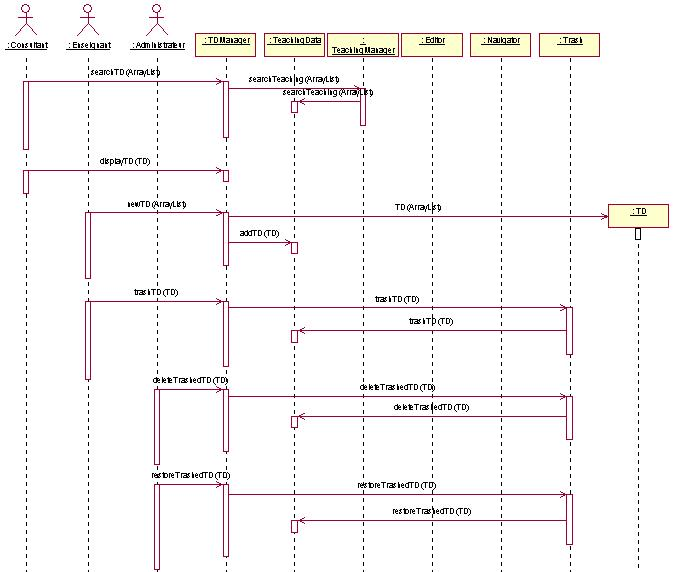
\includegraphics{images/td.jpg}}\\
\par Diagramme de s�quence des TD\\
\end{center}
